%%%%%%%%%%%%%%%%%%%%%%%%%%%%%%%%%%%%%%%%%%%%%%%%%%%%%%%%%%%%%%%%%%%%%%%%%%
% Information about mathematical background on backbone and implementation
%%%%%%%%%%%%%%%%%%%%%%%%%%%%%%%%%%%%%%%%%%%%%%%%%%%%%%%%%%%%%%%%%%%%%%%%%%

\chapter{Modelling Background} 
    \label{Modelling background}
    
In this chapter, the theoretical background of the implementation as outlined in chapter \ref{implementation} is described. The chapter is divided in several sections that each describe the different steps of modelling the fish's anatomy. To prevent confusions about terms concerning positions across the fish's body, a definition of the fish's anatomical axes is introduced in paragraph \ref{axes}. Then, the description of the formalization of \textit{Apteronotus leptorhynchus'} anatomy follows. The first is to represent its backbone as a parameterised curve that forms either a straight line or a curve turned at one point by a given angle. This curve was the basis for the cross-sections which were placed perpendicular to the backbone. How this orthogonality was achieved, is described in detail in paragraph \ref{crosssectional planes}. The last paragraph, \ref{Cross sections}, deals with the form of the cross sections themselves, that were modelled with the sum of an ellipsis and a variation of the Lorenz curve.

\section{Definition of Anatomical Axes}
    \label{axes}
    
In general, one describes the anatomical position in vertebrates using three axes. Depending on the specific animal the terms describing these axes vary. Therefore, we want to define the terms for the planes of the fish's anatomy in this paragraph to avoid misunderstandings. 

We use the terminology suggested by \citeA{harder1976anatomy} illustrated in Figure \ref{fig:Axes}. The first plane and with that the first axis is the \textit{horizontal} plane. It divides the fish into a dorsal and a ventral part along the fish's long axis. Perpendicular to the horizontal axis is the \textit{median} plane that is also positioned along the fish's long axis. It is the only plane that divides the fish into two nearly symmetrical halves that may be termed \textit{left} and \textit{right} half, respectively. The last plane is positioned perpendicular to both other planes and is called the \textit{transverse} plane. It cuts the fish at the middle of the long axis into a \textit{cranial} and a \textit{caudal} part. \\

\begin{figure}
   \centering
   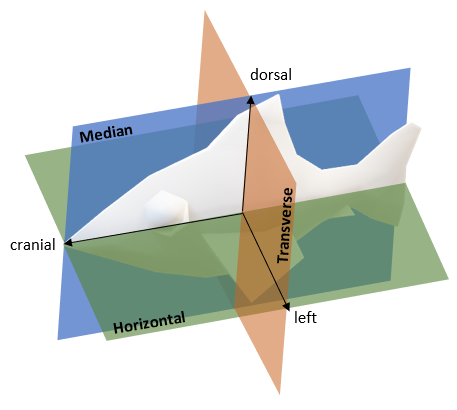
\includegraphics[width=10cm]{figures/Axes.PNG}
   \caption{Visualisation of a fish's axes. The median plane is depicted in blue, the horizontal plane in green and the transverse plane in red.}
   \label{fig:Axes}
\end{figure}

In the following chapters, various sections along one of the axes are used for the anatomical model. Their terminology is straightforward from the axes' terminology, but will be shortly defined here nevertheless: there are \textit{horizontal, median} and \textit{transverse} sections, respectively. Sections which are not positioned along one axis but rather parallel to it, are termed \textit{parahorizontal, paramedian} or \textit{paratransverse}. To shorten the term of the paratransverse section, that is used frequently in the following sections, we simply refer to them as \textit{cross-sections}.

\section{Backbone}
    \label{BackboneModelling}
    
The first step in modelling \textit{Apteronotus leptorhynchus'} anatomy consisted in modelling its backbone. This was done by describing a curve that can be, on the one hand, a straight line, if the fish does not bend its tail. And, on the other hand, bending should be possible, as specimen of \textit{Apteronotus leptorhynchus} do that to alter the spatial relation between their electric organ and their electroreceptors across the whole body \cite{bell1997generation}. Similar movements have been observed in \textit{Marcusenius cyprinoides} that belong to the family of Mormyriformes that also use active electrolocation as described in the introduction. Their exploration behaviour is visualized in Figure
\ref{ExplorationBehaviour} to get a more exact impression of the movements that were considered while modelling.

The horizontal coordinate, in the following represented by the $z$-coordinate, is kept constantly at $0$, because the fish does not move its body up- or downwards but keeps it rather straight or bent only in $x$- and $y$-direction, i.e. inside the plane spanned by transverse and median axis. 

\begin{figure}
   \centering
   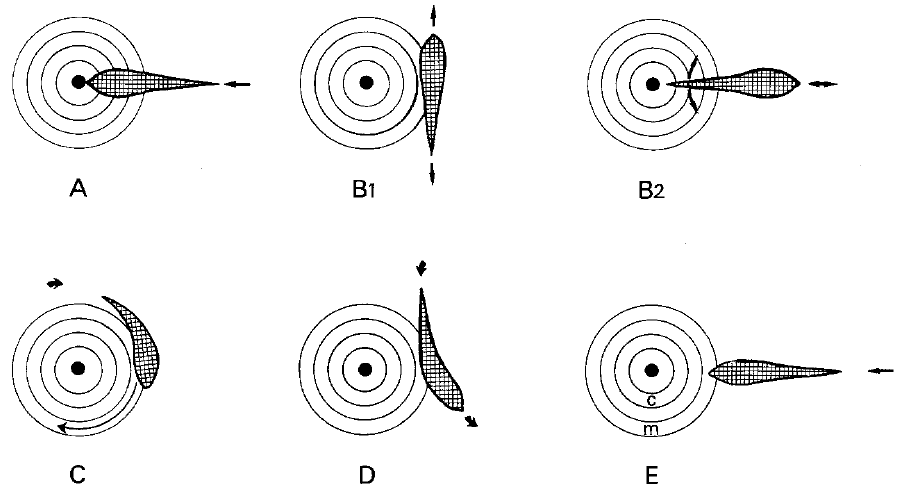
\includegraphics[width=10cm]{figures/ExplorationBehaviour.png}
   \caption{Exploration behaviour of \textit{Marcusenius cyprinoides} taken from \cite{toerring1979motor}. The different body shapes the fish uses in order to explore an object suggests, that an anatomical model of this species should provide various underlying backbone forms: as straight backbone and a curved one. If \textit{A. leptorhynchus} use the same behaviour, which is unknown by now, a model of this species' anatomy should offer the same possibilities. }
   \label{ExplorationBehaviour}
\end{figure}

A step-wise modulation of the fish's tail-bending behaviour is therefore necessary to model the temporally specific electric fields.
This was modelled with a curve that includes one turning point as this describes the fish's body position in a sufficient way. A hyperbola that suffices this criterion is visualized in Figure \ref{Backbonefunction}.
\begin{figure}[ht]
   \centering
   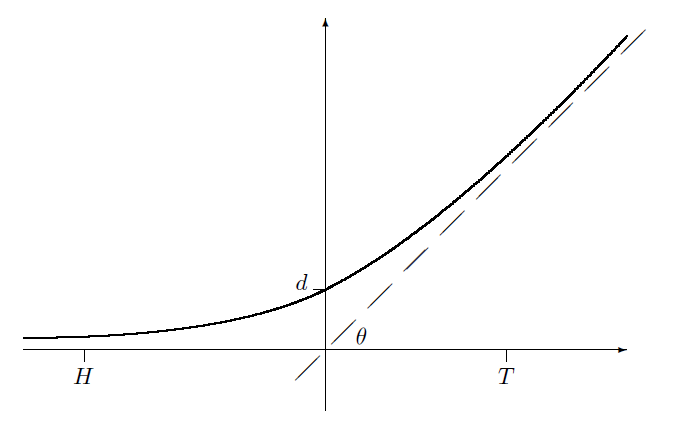
\includegraphics[width=10cm]{figures/BackboneFunction.PNG}
   \caption{The illustrated hyperbola models the fish's backbone as seen from above the fish, the horizontal axis is not visible. $H$ is the fish's head's transverse position, $T$ its tail's transverse position. $d$ specifies the median coordinate of the intersection between curve and median axis. The hyperbola converges to two asymptotes: The first one being the transverse axis, the second being a straight line from the origin with angle $\theta$ to the median axis.}
   \label{Backbonefunction}
\end{figure}

The hyperbola tends to two asymptotes at its limits. The first asymptote is the negative $x$-axis that represents the transverse axis while the other asymptote is given by a straight line with angle $0 \leq \theta < 90°$ from the $x$-axis. In the mathematical description of the hyperbola, the slope of the second asymptote is defined by $a := tan(\theta)$. The fish's head $H$ and due to that also the tail $T$ may be shifted along the $x$-axis to change the point at which the tail is bent, because the intersection with the y-axis (median axis), $d$, influences the curvature as well.
The equation for the hyperbola $f:\mathbb{R} \rightarrow \mathbb{R}$ is given by 
\begin{flalign}
f(x) = \frac{1}{2} \cdot (ax + \sqrt{4d^2 + a^2x^2}).
\end{flalign}

\newpage
To represent this equation in a parameterised planar curve depending only on the length parameter $l$, let $c: \mathbb{R} \rightarrow \mathbb{R}^2$ be:
\begin{flalign}
c(x) := \begin{pmatrix} x \\ f(x) \end{pmatrix}
\end{flalign}

Then one applies the general formula for the length of a parameterised curve as defined by \citeA[Def. 2.1.15]{bar2010elementare}
\begin{flalign}
l := \int_a^b{\norm{c'(x)} dx}
\end{flalign}
to $c$, with $H$ specified as the head's position. $c'(x)$ represents the first derivative of $c$. $s(b)$ then describes the length from the fish's head to the given transverse position $b$:
\begin{flalign}
l = s(b) = \int_H^b \sqrt{1+(f'(x))^2} dx.
\label{eq:s_x}
\end{flalign}

The parameterisation is necessary for further steps in modelling the fish's anatomy as described in the following paragraphs. 
Given a specific point $l$ on the backbone, its three-dimensional position is then described by $B(l): \mathbb{R} \rightarrow \mathbb{R}^3$:
\begin{flalign}
B(l) := \begin{pmatrix} s^{-1}(l) \\ f(s^{-1}(l)) \\ 0 \end{pmatrix}.
\label{eq:3dvector}
\end{flalign}

As mentioned before, the $z$-coordinate and with that the coordinate on the horizontal axis is kept constantly at $0$ because the fish does not move its body up- or downwards.

\section{Cross-sectional Planes}
    \label{crosssectional planes}
    
To be able to translate and turn the two-dimensional cross-sectional points resulting from the MRI data into three dimensions, it is first obligatory to define the Frenet-coordinate frame at each point along the backbone. Thus, the three vectors specifying the coordinate frame need to be defined in a general form depending on $l$, the point on the backbone. The tangent vector, $\vec{e_1}$, points along the fish's body axis, the normal vector, $\vec{e_2}$, points to its left and the binormal vector, $\vec{e_3}$, upwards. The $z$-coordinates of the hyperbola are kept constantly at $0$ and due to that the torsion $\tau$ as well. As a result, $\vec{e_3}$ is not dependent on $l$ and stays the same along the whole backbone. Following these characterestics, the unit Frenet vectors are given by
\begin{flalign}
\vec{e_1}(x) = \frac{c'(x)}{||c'(x)||}, \vec{e_2}(x) = \frac{\vec{e_1}'(x)}{||\vec{e_1}'(x)||}, \vec{e_3}(x) = \begin{pmatrix} 0 \\ 0 \\ 1 \end{pmatrix}. 
\end{flalign}

Using the definition of $B(l)$ from equation \ref{eq:3dvector}, that leads to
\begin{flalign}
\vec{e_1}(l) = \begin{pmatrix} 1 \\ f'(s^{-1}(l)) \\ 0\end{pmatrix} \cdot \frac{1}{||B'(l)||}
\end{flalign}

and
\begin{flalign}
\vec{e_2}(l) = \begin{pmatrix} f'(s^{-1}(l)) \\ -1 \\ 0\end{pmatrix} \cdot \frac{1}{||\vec{e_1}(l)||}.
\end{flalign}

Using these definitions, one can construct the plane containing $\vec{e_2}$ and $\vec{e_3}$, so the normal and the binormal vector called the normal plane. The normal planes determine how exactly the cross-sections need to be positioned -- such that they are contained in the corresponding normal plane. Thus, a transformation from the two-dimensional points of the cross-sections to three-dimensional points lying inside the normal planes is necessary. One way, how this can be achieved, is described in subsection \ref{relativeposition}.

\section{Cross-sections}
    \label{Cross sections}
    
Having calculated the Frenet-coordinate frame, it is now necessary to model the cross-sections themselves. \\
The form of the cross-sections varies slightly along the fish's long axis, implying that cross-sections located in the cranial part differ from the ones in the caudal part and from the ones close to the center. The forms resemble an ellipsis at the fish's head and become more and more pointed towards its tail. Example cross-sections from the fish's head, center and tail can be seen in Figure \ref{fig:crosssections}.

\begin{figure}
    \centering
    \begin{minipage}[t]{0.32\textwidth}
    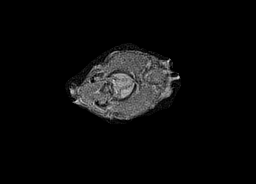
\includegraphics[width=\textwidth]{figures/cs12.png}
    \caption*{a)}
    \end{minipage}
    \begin{minipage}[t]{0.32\textwidth}
    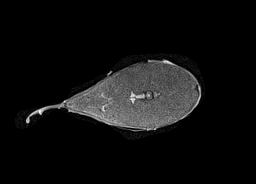
\includegraphics[width=\textwidth]{figures/cs62.png}
    \caption*{b)}
    \end{minipage}
    \begin{minipage}[t]{0.32\textwidth}
    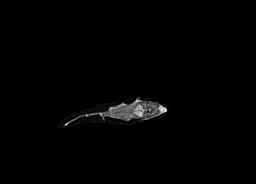
\includegraphics[width=\textwidth]{figures/cs114.png}
    \caption*{c)}
    \end{minipage}
    \caption{Cross-sections from MRI-data: \textbf{a)} close to fish's head (12 mm caudal to head), \textbf{b)} close to fish's transverse plane (62 mm caudal to head, 66 mm cranial to tail), \textbf{c)} close to fish's tail (14 mm cranial to tail). The fish had a total length of 128 mm.}
    \label{fig:crosssections}
\end{figure}

Following from these varying forms, one needs a function describing an ellipsis as its basic form and a factor that defines the tail's shape. Again, we want it to be in parameterised form to define the cross-section relative to the point on the backbone depending on the angle $\varphi$. Hence, we use the parameterised form of an ellipsis and add a factor close to the parameterised Lorenz curve to it. Taking all that into account, we get:

\begin{flalign}
r(\varphi) = \sqrt{\frac{a^2 b^2}{a^2 \cdot cos^2(\varphi) + b^2 \cdot sin^2(\varphi)}} + \frac{m}{(\varphi - \pi)^2+2}.
\label{eq:ellipsis}
\end{flalign}

$r(\varphi)$ specifies the distance from the origin at angle $\varphi$. With different values of $a$, $b$ and $m$ it is then possible to approximate the contours of the individual cross-sections.
